\documentclass[a4paper,10pt]{article}
\usepackage[margin=1in]{geometry}
\usepackage[showframe=true]{geometry}
\usepackage{changepage}
\usepackage{polski}
\usepackage[utf8x]{inputenc}
\usepackage[unicode]{hyperref}
\usepackage{amssymb}
\usepackage{xifthen}
\usepackage[fleqn]{amsmath}
\usepackage{todonotes}
\usepackage{graphicx}
\usepackage{float}
\usepackage{fullpage}
\usepackage{epstopdf}
\usepackage{multirow}
\usepackage{subfig}
\usepackage{booktabs}
\usepackage[europeanresistors,americaninductors]{circuitikz}
\usetikzlibrary{patterns}
\newcommand{\withtodo}{0}

\def\arraystretch{1}

\begin{document}

\begin{table}
  \centering
  \def\arraystretch{1.5}
    \begin{tabular}{|l|l|l|l|} \hline
    Wydział:           & \multicolumn{2}{l|}{Dzień:Poniedziałek 14-17}    &Zespół:  \\
    Fizyki             &    \multicolumn{2}{l|}{Data: 20.03.2017}         &8             \\\hline
    Imiona i nazwiska: &Ocena z przygotowania:  &Ocena ze sprawozdania:   &Ocena końcowa: \\
    Marta Pogorzelska  &                        &                         &                \\
    Paulina Marikin    &                        &                         &\\\hline
    \multicolumn{2}{|l|}{Prowadzący:                 } &\multicolumn{2}{l|}{Podpis:             }  \\\hline
  \end{tabular}
\end{table}


\title{Ćwiczenie 3:\\Wahadło matematyczne}
\date{}
\maketitle{}

\section{Cel badań}
Zbadanie zjawiska anharmoniczności drgań wahadła matematycznego, tj: zależności okresu drgań wahadła od kąta wychylenia oraz wyznaczenie wartości przyspieszenia ziemskiego przy użyciu wahadła różnicowego.

\section{Wstęp teoretyczny}
Wahadłem matematycznym jest ciało o masie punktowej m, zawieszone na cienkiej, nieważkiej lince, poruszające się po okręgu w jednorodnym polu grawitacyjnym.
\\
\begin{figure}[H]
\centering
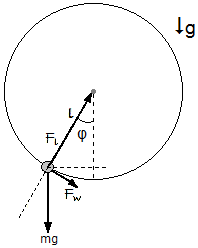
\includegraphics[width=0.15\textwidth]{wahadlo.png}
\caption{Wahadło matematyczne}
\end{figure}.
\\
\\Ciało porusza się po okręgu wychylając się z położenia równowagi o pewien kąt  i zakreślając łuk o długości:
\begin{equation}
S = l\varphi
\end{equation}
,gdzie l - odległość punktu materialnego od osi obrotu, $\varphi$ - kąt wychylenia wahadła
\\ Równanie ruchu dla takiego ciała ma postać:
\begin{equation}
m\frac{d^2S}{dt^2} = -mg\sin\varphi
\end{equation}
\\Po podstawieniu wzoru (1) do równania (2) otrzymujemy i dodaniu stronami:
\begin{equation}
\frac{d^2\varphi}{dt^2} + \frac{g}{l}\sin\varphi = 0
\end{equation}
\\Rozwiązaniem tego równania dla ruchu oscylującego i jednocześnie wzorem na okres drgań wahadła jest:
\begin{equation}
T(\varphi) = 2\pi\sqrt{\frac{l}{g}}\sum_{n=0}^{\infty}\bigg(\frac{(2n)!}{(2^nn!)^2}\bigg)^2\sin^{2n}\bigg(\frac{\varphi}{2}\bigg)
\end{equation}
\\Jest to jednak równanie czyste teoretyczne i nie ma podejści apraktycznego, gdyż liczba zliczeń dąży do nieskończoności. W przeprowadzanym doświadczeniu kąt wychylenia jest nieduży ($\varphi<\frac{\pi}{2}$). Dla dokładnośći 3 miejsc znaczących wystarczy branie pod uwagę jedynie sumy dla n=3. Po podstawieniu tych zależności do wzoru (2) otrzymujemy:
\begin{equation}
T(\varphi) = 2\pi\sqrt{\frac{l}{g}}\bigg(1+\frac{1}{4}\sin^2\frac{\varphi}{2}+\frac{9}{64}\sin^4\frac{\varphi}{2}+\frac{25}{256}\sin^6\frac{\varphi}{2}\bigg)
\end{equation}
\\Dla wyznaczenie wartości przyspieszenia ziemskiego należy zmierzyć 3 wielkości: kąt wychylenia wahadła $\varphi$, okres jego drgań T oraz długość linki l. To ostatnie jest jednak trudne do wykonania w warunkach laboratoryjnych ze względu na trudność wyznaczenia środka masy soczewki wahadła. W tym celu wykorzystana zostanie metoda obliczeń dla wahadła różnicowego, gdzie dokonuje się pomiaru zmiany długości wahadła($l_i, l_j$ - dwie różne długości wahadła). Wzór (5) ma wtedy postać:
\begin{equation}
T_i(\varphi) = 2\pi\sqrt{\frac{l_i}{g}}f^2(\varphi)\\\\\\
T_j(\varphi) = 2\pi\sqrt{\frac{l_j}{g}}f^2(\varphi)
\end{equation}
,gdzie $f(\varphi)=\sum_{n=0}^{\infty}\bigg(\frac{(2n)!}{(2^nn!)^2}\bigg)^2\sin^{2n}\bigg(\frac{\varphi}{2}\bigg)$; $T_i, T_j$ - okresy drgań wahadła zmierzone dla kolejnych długości nici $l_i, l_j$.
\\
\\Po podniesieniu do kwadratu wzorów (6) i odjęciu stronami dostajemy:
\begin{equation}
T_i^2-T_j^2 = \frac{4\pi^2}{g}(l_i-l_j)f^2(\varphi)
\end{equation}

\section{Opis układu i metody pomiarowej}
Aparatura pomiarowa
\begin{itemize}
  \item model wahadła matematycznego
\begin{itemize}
  \item statyw
  \item metalowe ciało o regularnym kształcie
  \item jedwabna nić
  \item czujka do mierzenia okreu
\end{itemize}
  \item elektroniczny układ pomiarowy z automatycznym pomiarem okresu
  \item linijka
\end{itemize}
 
\subsection{Badanie zależności okresu drgań wahadła od kąta wychylenia}
Najpierw wykonano pomiar długości linki przy użyciu linijki od środka masy kulki do punktu zaczepienia  i włączono stoper, który nastawiono na  pomiar 3 okresów. 
\begin{equation}
T_{sr} = \frac{t}{n}
\end{equation}
,gdzie $T_{sr}$ - średni okres drgań wahadła, t - czas n wachnięć wahadła
\\
\\Następnie odchylono kulkę o kąt $10\,^{\circ}$ od położenia równowagi i puszczono tak, by poruszała się równolegle do kątomierza na statywie. Na koniec złapano kulkę i spisano wynik z urządzenia oraz kąt odchylenia kulki po jej złapaniu. Czynność powtórzono pięciokrotnie, a pomiary wykonano dla kątów odchylenia  $10\,^{\circ}, 20\,^{\circ}, 30\,^{\circ}$ i $40\,^{\circ}$.

\subsection{Wyznaczenie wartości przyspieszenia ziemskiego}
W tej części doświadczenia wykonane zostały pomiary okresów dla stałego kąta wychylenia, ale dla różnych długości linki wahadła. Przyjęto stały, mały kąt $15\,^{\circ}$ i wykonano ćwiczenie analogicznie do poprzedniego. Długość odczytano z linijki na statywie, ponieważ do obliczeń potrzebna jest jedynie zmiana w długości wahadła, a nie odległość względem pewnego punktu odniesienia. Pomiary wykonano dla odczytów 50cm, 40cm, 30cm, 20cm, 10cm i 1,5cm. Do obliczeń korzystano ze wzoru (7).

\section{Wyniki i analiza pomiarów}
\subsection{Wahadło matematyczne $l=50(0.5)cm$}
\begin{tabular}{lrrrr}
\toprule
{$\varphi[^\circ]$} & 10.0(1.2) & 20.0(1.2)&  30.0(1.2)&40.0(1.2)\\
\midrule
4 okresy [s]&  4.9223(0.0001) &  5.7827(0.0001) &  5.7889(0.0001) &  5.8451(0.0001) \\
    &  5.6868(0.0001) &  5.7221(0.0001) &  5.7733(0.0001) &  5.8451(0.0001) \\
    &  4.9163(0.0001) &  5.7227(0.0001) &  5.7745(0.0001) &  5.8525(0.0001) \\
    &  5.6908(0.0001) &  5.7202(0.0001) &  5.7716(0.0001) &  5.8456(0.0001) \\
    &  4.9222(0.0001) &  5.7210(0.0001) &  5.7750(0.0001) &  5.8459(0.0001) \\\hline
średnia(std)[s]& 5.22(0.42) & 5.733(0.027) & 5.7766(0.0069) & 5.8468(0.0031)		\\\hline
1	okres[s]&	1.30(0.42) & 1.433(0.027) & 1.4441(0.0069) & 1.4617(0.0031) \\\hline
teoretyczny okres[s] & 1.421(0.012) & 1.4293(0.0094) & 1.443(0.012) & 1.462(0.015)\\
\bottomrule
\end{tabular}
\begin{figure}[H]
    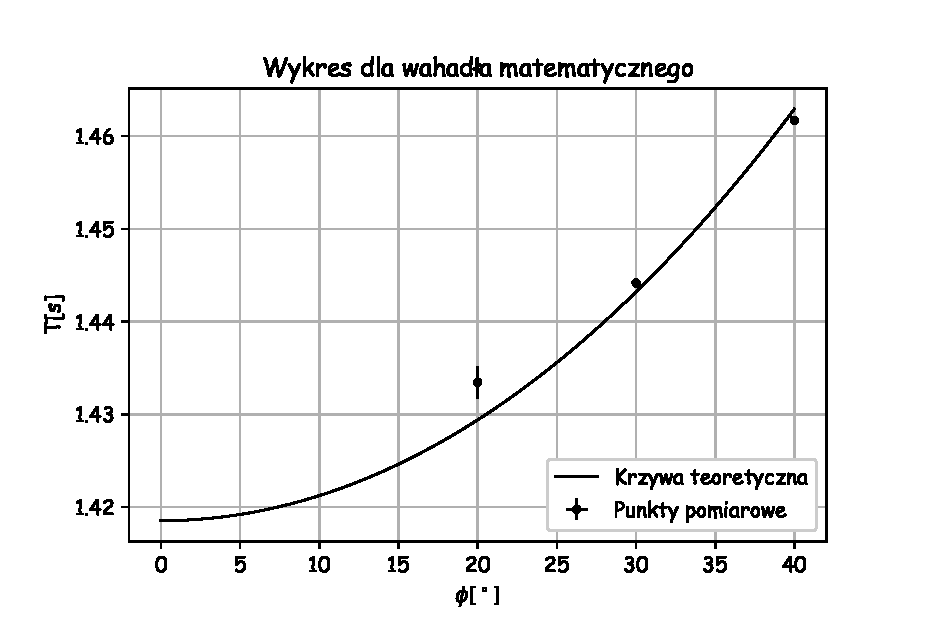
\includegraphics{./Wykres_matematyczne.eps}
    \caption{}
    \label{}
\end{figure}
Z pomiarów czasu dla wszystkich serii dla obu wahadeł wyciągnięto średnią. Pomiary dla wahadła matematycznego zostały podzielone na cztery w celu uzyskania pojedyńczego okresu. Krzywą teoretyczną wyliczono ze wzoru (3). Pomiar dla 10$^\circ$ został wyżucony jako błąd gruby, ze względu na dużą (ponad 15 razy większą niż pozostałe) niepewność. Pomiary dla pozostałych trzech rozważanych kątów leżą na krzywej teoretycznej w granicach swoich niepewności.

\subsection{Wahadło różnicowe $\varphi = 15^\circ$}
\begin{figure}[H]
\begin{adjustwidth}{-2cm}{}
\begin{tabular}{lrrrrrr}
\toprule
l[cm] &  50 &  40 &   30 &   20 &   10 &  1.5 \\
\midrule
t[s] &  1.2158(0.0001) &  1.3703(0.0001) &  1.5107(0.0001) &  1.6406(0.0001) &  1.7587(0.0001) &  1.8516(0.0001) \\
 &  1.2122(0.0001)&1.3690(0.0001)&1.5121(0.0001)&  1.6403(0.0001) &  1.7599(0.0001) &  1.8525(0.0001) \\
 &  1.2103(0.0001)&1.3705(0.0001)&1.5118(0.0001)&  1.6403(0.0001) &  1.7605(0.0001) &  1.8518(0.0001) \\
 &  1.2121(0.0001)&1.3703(0.0001)&1.5124(0.0001)&  1.6402(0.0001) &  1.7597(0.0001) &  1.8516(0.0001) \\
 &  1.2126(0.0001)&1.3706(0.0001)&1.5124(0.0001)&  1.6408(0.0001) &  1.7599(0.0001) &  1.8518(0.0001) \\
 &  1.2136(0.0001)&1.3704(0.0001)&1.5120(0.0001)&  1.6400(0.0001) &  1.7605(0.0001) &  1.8523(0.0001) \\\hline
T[s] &  1.2127(0.0019) & 1.37018(0.00082)  & 1.51190(0.00085)  & 1.64036(0.00064)  & 1.75986(0.00087)  
& 1.85193(0.00068) & \\\hline
$T^2[s^2]$ &  1.4708(0.0046) & 1.8774(0.0022)  & 2.2858(0.0025)  & 2.6908(0.0021)  & 3.0971(0.0030)  & 3.4296(0.0025) & \\
\bottomrule
\end{tabular}
 \end{adjustwidth}
\end{figure}

\begin{figure}[H]
    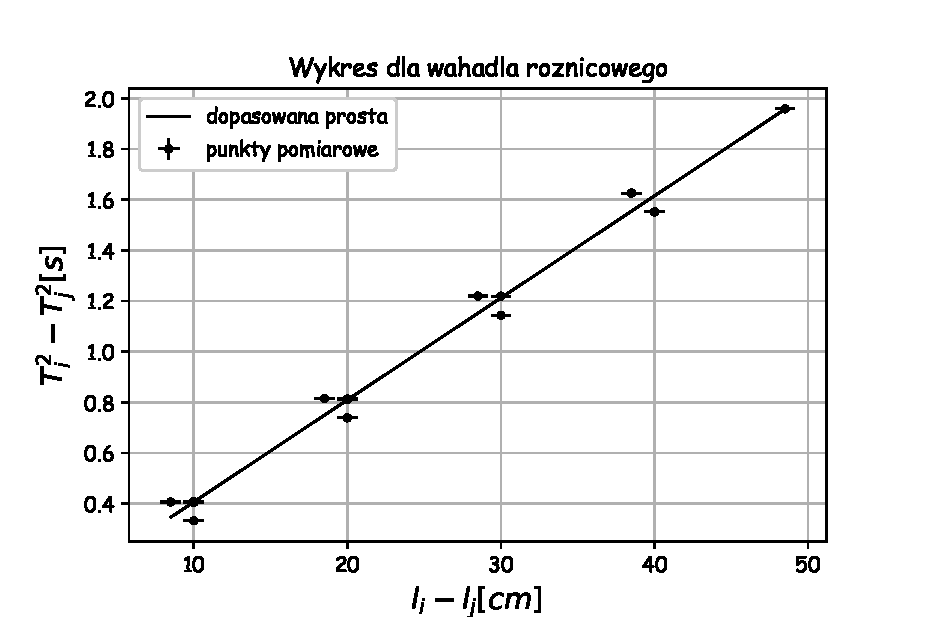
\includegraphics{./Wykres_roznicowe.eps}
    \caption{}
    \label{}
\end{figure}
Pomiary zostały opracowane zgodnie ze wzorem (7), od każdego pomiaru długości (i kwadratu odpowiadającego mu pomiaru okresu) odjęto wszystkie pomiary odeń mniejsze. Otrzymane różnice przedstawiono na wykresie wraz z dopasowaną do nich prostą. Prosta zostałą dopasowana funkcją \emph{polyfit} pakietu \emph{numpy} 
w Pythonie.\\
$a = 0.0402878(0.0000015)$
\\ 
Parametr kierunkowy dopasowanej prostej został przyrównany do pozostałej części zależności (7):
\begin{equation}
a = \frac{4 \pi^2}{g} f(\varphi)
\end{equation}
gdzie a - parametr kierunkowy. Przekształcenie powyższej równości pozwoliło na wyliczenie przyspieszenia ziemskiego, którego wyliczona wartość wynosi g = 9.841(0.299)[$\frac{m}{s^2}$]
\section{Analiza niepewności}
Niepewność pomiarów to:
\begin{itemize}
	\item długość $\Delta l = 0.5 cm$
	\item czas $\Delta T = 0.001 s$
	\item kąt $\Delta \varphi = 2 ^\circ$
\end{itemize}
Dla wszystkich okresów przy wyliczaniu niepewności wzięto pod uwagę także ich odchylenie standardowe. 
$$\mu(T) = \sqrt{std^2 + \frac{\Delta T^2}{3}}$$
Zarówno dla długości jak i dla kąta do niepewności doliczono niepewność eksperymentatora równa połowie niepewności pomiaru
$$\mu(x) = \sqrt{\frac{\Delta x^2}{3}+\frac{(\frac{\Delta x}{2}})^2{3}}$$
Niepewność dopasowanej prostej stanowi pierwiastek kowariancji zwracanej przez funkcję \emph{polyfit} pakietu \emph{numpy} w Pytonie. Dla g niepewność wyliczono metodą propagacji niepewności:
$$\mu(g) = \sqrt{(\Delta a \frac{4 \pi^2 f(\varphi)}{a^2})^2+(\Delta f(\varphi) \frac{4 \pi^2}{a})^2}$$
\section{Wnioski}
Okres wahadła matematycznego jest zależny od kąta wychylenia. Wysoka (w zakresie jednego przedziału niepewości) zgodność większości punktów pomiarowych do krzywej teoretycznej skłania do potwierdzenia, iż badna teoria poprawnie opisuje daną zależność. Pomiar dla $10^\circ$ wydaje się być niepoprawny ze względu na dużą (w porównaniu z innymi niepewność) i jego odchylenie od krzywej nie musi wskazywać na niepoprawność tezy. Jednak cztery, a tym bardziej trzy punkty pomiarowe to dość mało. By potwierdzić tezę należałoby wykonać pomiary dla większej ilości kątów wychyleń.\\
\\
Badana zależność dla wahadła różnicowego wyraźnie wykazuje charakter liniowy. Wyznaczone przyspieszenie ziemskie jest zbliżone do tablicowego. %Można by coś dopisać o kształcie tego wykresu. Bo ustawienie punktów jest dziwnie powtarzalne i symetryczne względem dopasowanej prostej 

\end{document}
